\documentclass[10pt]{article}
\usepackage[]{ragged2e}
\usepackage{fancyhdr,amsmath,amsthm,amssymb,bbm,graphicx}
\usepackage[utf8]{inputenc}
\usepackage[letterpaper,left=25mm,right=25mm]{geometry}

\setlength{\parskip}{1em}
\setlength{\parindent}{0em}

\newcommand{\Z}{\mathbb{Z}}
\newcommand{\R}{\mathbb{R}}
\newcommand{\Q}{\mathbb{Q}}
\newcommand{\C}{\mathbb{C}}
\newcommand{\N}{\mathbb{N}}

\DeclareMathOperator{\Ima}{Im}

\linespread{1.25}
\pagestyle{fancy}
\fancyhf{}
\lhead{PHYS 442 $|$  Assignment 1}

\rhead{Dilraj Ghuman $|$ 20564228}

\begin{document}

\begin{figure}
  \centering
  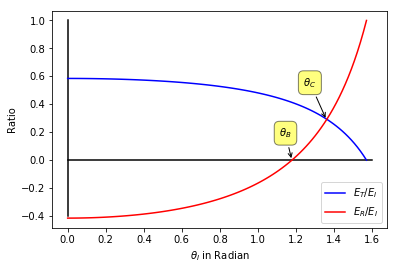
\includegraphics[scale=0.8]{ET_ER_plot.png}
  \caption{A plot of the ratio of transimitted wave to the incident and the reflected wave to the incident. We see that we have labled the brewster's angle and the angle at which we have conversion between the two.}
\end{figure}

\begin{figure}
  \centering
  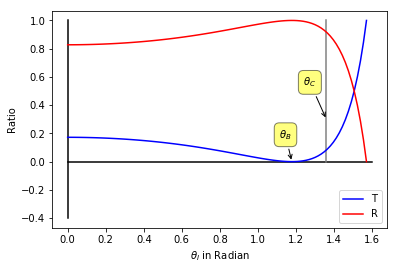
\includegraphics[scale=0.8]{T_R_plot.png}
  \caption{A plot of the transmitted and reflected amplitudes.}
\end{figure}

\end{document}
